\documentclass[]{book}

%These tell TeX which packages to use.
\usepackage{array,epsfig}
\usepackage{amsmath}
\usepackage{amsfonts}
\usepackage{amssymb}
\usepackage{amsxtra}
\usepackage{amsthm}
\usepackage{mathrsfs}
\usepackage{color}
\usepackage{graphicx}
\usepackage{bm}
\usepackage{tikz}
%\usepackage{widthof}
\usetikzlibrary{arrows}

%Here I define some theorem styles and shortcut commands for symbols I use often
\theoremstyle{definition}
\newtheorem{defn}{Definition}
\newtheorem{thm}{Theorem}
\newtheorem{cor}{Corollary}
\newtheorem*{rmk}{Remark}
\newtheorem{lem}{Lemma}
\newtheorem*{joke}{Joke}
\newtheorem{ex}{Example}
\newtheorem*{soln}{Solution}
\newtheorem{prop}{Proposition}

\newcommand{\lra}{\longrightarrow}
\newcommand{\ra}{\rightarrow}
\newcommand{\surj}{\twoheadrightarrow}
\newcommand{\graph}{\mathrm{graph}}
\newcommand{\bb}[1]{\mathbb{#1}}
\newcommand{\Z}{\bb{Z}}
\newcommand{\Q}{\bb{Q}}
\newcommand{\R}{\bb{R}}
\newcommand{\C}{\bb{C}}
\newcommand{\N}{\bb{N}}
\newcommand{\M}{\mathbf{M}}
\newcommand{\m}{\mathbf{m}}
\newcommand{\MM}{\mathscr{M}}
\newcommand{\HH}{\mathscr{H}}
\newcommand{\Om}{\Omega}
\newcommand{\Ho}{\in\HH(\Om)}
\newcommand{\bd}{\partial}
\newcommand{\del}{\partial}
\newcommand{\bardel}{\overline\partial}
\newcommand{\textdf}[1]{\textbf{\textsf{#1}}\index{#1}}
\newcommand{\img}{\mathrm{img}}
\newcommand{\ip}[2]{\left\langle{#1},{#2}\right\rangle}
\newcommand{\inter}[1]{\mathrm{int}{#1}}
\newcommand{\exter}[1]{\mathrm{ext}{#1}}
\newcommand{\cl}[1]{\mathrm{cl}{#1}}
\newcommand{\ds}{\displaystyle}
\newcommand{\vol}{\mathrm{vol}}
\newcommand{\cnt}{\mathrm{ct}}
\newcommand{\osc}{\mathrm{osc}}
\newcommand{\LL}{\mathbf{L}}
\newcommand{\x}{\bm{x}}
\newcommand{\UU}{\mathbf{U}}
\newcommand{\support}{\mathrm{support}}
\newcommand{\AND}{\;\wedge\;}
\newcommand{\OR}{\;\vee\;}
\newcommand{\Oset}{\varnothing}
\newcommand{\st}{\ni}
\newcommand{\wh}{\widehat}

%Pagination stuff.
\setlength{\topmargin}{-.3 in}
\setlength{\oddsidemargin}{0in}
\setlength{\evensidemargin}{0in}
\setlength{\textheight}{9.in}
\setlength{\textwidth}{6.5in}
\pagestyle{empty}



\begin{document}


\begin{center}
{\Large Draft}\\
\textbf{Alireza Abrehforoush}\\ %You should put your name here
Date: 7-27-2022 %You should write the date here.
\end{center}
\vspace{0.2 cm}


\section{Part 1 (2nd\hspace{0.1cm} approach)}
\subsection{Model}
We model the problem with three systems $0$, $1$ and $2$ corresponding to the following set of states of $\left\{ n \right\}$, $\left\{0, n-2\right\}$ and $\left\{1,2,3,\hdots,n-3\right\}$ of previous model respectively. We denote the upper bound of stay of our random walker on expectation in system $i$ by $T_{i}$. 

%graph
\begin{center}
\begin{tikzpicture}
\tikzset{vertex/.style = {shape=circle,draw,minimum size=3em}}
\tikzset{edge/.style = {->,> = latex'}}
% vertices
\node[vertex] (a) at  (0,1.5) {$0^{\prime}$};
\node[vertex] (b) at  (0,0) {$1^{\prime}$};
\node[vertex] (c) at  (0,-1.5) {$2^{\prime}$};
%edges
\draw[->] (a) edge  [loop above] node {$1$} ();
\draw[->] (b) edge  [loop right] node {$1-3p$} ();

\path[->] (b) edge
node[right]{$p$} (a);
\path[->] (b) edge[bend right]      node[left]{$2p$} (c);
\path[->] (c) edge[bend right]      node[right]{$q$} (b);

\draw[->] (c) edge  [loop below] node {$1-q$} ();

\end{tikzpicture}
\end{center}
%graph

We compute an upper bound for expected equilibrium time starting from any arbitrary system ($T$).

\begin{equation}\label{}
\begin{split}
    T &= p\times \left(T_{2} + 2\right) \\
      &+ p\times \left(2T_{2} + 4\right)\times 2p \\
      &+ p\times \left(3T_{2} + 6\right)\times \left(2p\right)^2 \\
      & \vdots \\
      &= \frac{1}{2p} \sum_{i=1}^{\infty} p i \left(T_{2} + 2\right)\left(2p\right)^i \\
      &= \frac{p\left(T_{2} + 2\right)}{\left(1-2p\right)^2}
\end{split}
\end{equation}

To calculate the value of $T_2$ we can use the settings that we had in the first approach.

%graph
\begin{center}
\begin{tikzpicture}
\tikzset{vertex/.style = {shape=circle,draw,minimum size=3em}}
\tikzset{edge/.style = {->,> = latex'}}
% vertices
\node[vertex] (a) at  (-6,0) {$0$};
\node[vertex] (b) at  (-2,0) {$1$};
\node[vertex] (c) at  (2,0) {$2$};
\node[vertex] (d) at  (6,0) {$n-2$};
%edges

\path[->] (a) edge[bend right]
node[below]{$2p$} (b);
\path[->] (b) edge[bend right]
node[above]{$2p$} (a);

\draw[->] (b) edge  [loop above] node {$1-4p$} ();

\path[->] (b) edge[bend right]      node[below]{$2p$} (c);
\path[->] (c) edge[bend right]      node[above]{$2p$} (b);

\draw[->] (c) edge  [loop above] node {$1-4p$} ();

\path (c) to node {\dots} (d);

\end{tikzpicture}
\end{center}
%graph

We consider states $1,2,\ldots,n-3$ corresponding to the configuration with $c = i \in \left\{0,1,\ldots,n\right\}$. 
Let $t_c$ denote the expected reaching time to state $0$ or $n-2$, starting from state $c$.
The changes in $c$ are governed by the following non-homogeneous linear recurrence relation
\begin{equation}    \label{mainEquation}
    t_c 
    = 2p t_{c-1}  + 2p t_{c+1} + (1 - 4p)t_{c} + 1\\
    = \frac{1}{2}t_{c-1} + \frac{1}{2}t_{c+1} + \frac{1}{4p}, \quad c = 1,\ldots,n-3,
\end{equation}
and following initial conditions
\begin{equation}\label{recursiveEquation_t_0}
    t_0 = 0 \qquad t_{n-2} = 0
\end{equation}

We solve the recurrence same way as the first approach. thus, the final closed form is:
\begin{equation} \label{closed form}
    t_c = \frac{c(n-c-2)}{4p}\\
\end{equation}

For every $c \in \left\{0, 1, 2, 3, \hdots, n-2\right\}$ we have:
\begin{equation*} \label{}
    t_c \le t_{\frac{n-2}{2}}
\end{equation*}
So
\begin{equation} \label{}
    T_2 = t_{\frac{n-2}{2}}
\end{equation}

By (1) and (5) we can infer that the expected equilibrium time would be at most 
\begin{equation}\label{}
\begin{split}
    \frac{p\left( \frac{\left(n-2\right)^2}{16p} + 2\right)}{\left(1-2p\right)^2}
\end{split}
\end{equation}
%%%%%%%%%%%%%%%%%%%%%%%%%%%%%%%%%%%%%%%%%%
\section{Extending 2nd approach to m systems}
\begin{figure}[ht]
    \centering
    \includegraphics[width=0.4\textwidth]{figures/3.jpg}
    \caption{configuration with 3 red arcs of length one, two and three}
    \label{fig:mesh1}
\end{figure}
For each set of configurations with same number of arcs, we consider a unique system that includes all these configurations. we denote the upper bound of stay of our random walker in system $i$ by \emph{$T_i$}. also \emph{$p_{i, j}$} denotes the probability of reaching from system $i$ to system $j$ in one step. and finally, \emph{$t_{i, j}$} denotes the reaching time to system $j$ for the first time, starting from system $i$.
%graph
\begin{center}
\begin{tikzpicture}
\tikzset{vertex/.style = {shape=circle,draw,minimum size=3em}}
\tikzset{edge/.style = {->,> = latex'}}
% vertices
\node[vertex] (a) at  (-6,0) {$0^{\prime}$};
\node[vertex] (b) at  (-2,0) {$1^{\prime}$};
\node[vertex] (c) at  (2,0) {$2^{\prime}$};
\node[vertex] (d) at  (6,0) {$\left\lfloor \frac{n}{2} \right\rfloor ^{\prime}$};
%edges

\path[->] (a) edge[bend left]
node[above]{$p_{0,1}$} (b);
\path[->] (b) edge[bend left]
node[below]{$p_{1,0}$} (a);
\path[->] (b) edge[bend left]
node[above]{$p_{1,2}$} (c);
\path[->] (c) edge[bend left]
node[below]{$p_{2,1}$} (b);
\path (c) to node {\dots} (d);


\end{tikzpicture}
\end{center}
%graph

 We may have following recurrence relation for $t$s:
\begin{equation}
\begin{split}
    t_{c, 0} = t_{c, c-1} + t_{c-1, c-2} + \hdots + t_{1, 0}
\end{split}
\end{equation}

\begin{equation}
\begin{split}
    t_{c, c-1} = p_{c, c+1} t_{c+1, c-1} + \left( 1 - p_{c, c+1} - p_{c, c-1} \right) t_{c, c-1} + p_{c, c-1} + 1
\end{split}
\end{equation}


%%%%%%%%%%%%%%%%%%%%%%%%%%%%%%%%%%%%%%%%%%
\section{New approach for main problem (asynchronous version) (probably similar to the phase transition paper)}
\subsection{Model}
For any configuration \emph{$c$} with $n$ agents there exists a string of $0$s and $1$s with length $n$, each $0$s and $1$s corresponding to black arc (equilibrium) and red arc (not equilibrium) respectively.
the activation of any agent between arcs $i$ and $i+1$ leads to one of the following modifications in the string:
\begin{center}
    \begin{table}[ht]
        \begin{tabular}{|l|l|}
        \hline
        00 & 11 \\ \hline
        01 & 10 \\ \hline
        10 & 01 \\ \hline
        11 & 11 \\ \hline
        \end{tabular}
    \end{table}
\end{center}

We denote the number of red arcs in configuration $c$ by $r(c)$. also we denote configuration in next step (current configuration is $c$) by $\delta(c)$.
We denote the $r(\delta(c)) - r(c)$ by $\Delta r$ and compute its expected value as follows:

\begin{equation}
\begin{split}
    \mathbb{E}[\Delta r] &= \mathbb{E}[\Delta r | \text{activation of agent between two red arcs}] \times \mathbb{P}\left\{ \text{activation of agent between two red arcs} \right\} \\
    &+ \mathbb{E}[\Delta r | \text{activation of agent not between two red arcs}] \times \mathbb{P}\left\{ \text{activation of agent not between two red arcs} \right\} \\
    &= -2\times \mathbb{P}\left\{ \text{activation of agent between two red arcs} \right\}
\end{split}
\end{equation}

If we have such a lower bound for $\mathbb{P}\left\{ \text{activation of agent between two red arcs} \right\}$ in any configuration, we can calculate an upper bound for the expected time of reaching to equilibrium through dividing number of red arcs by $\mathbb{E}[\Delta r]$. (failed. because it can be zero :( )

\end{document}